% Comparación de curvaturas K<0, K=0, K>0
% Visualización mediante abanicos de geodésicas (ecuación de Jacobi)
% Compilar con: pdflatex curvature_comparison.tex
\documentclass[tikz,border=10pt]{standalone}
\usepackage{tikz}
\usepackage{xcolor}
\definecolor{gdlblue}{RGB}{41, 98, 168}
\definecolor{gdlred}{RGB}{191, 49, 49}
\definecolor{gdlgreen}{RGB}{30, 130, 76}
\definecolor{gdlorange}{RGB}{217, 130, 30}
\definecolor{gdlpurple}{RGB}{118, 56, 138}
\definecolor{gdlgray}{RGB}{140, 140, 140}
\definecolor{gdlyellow}{RGB}{190, 140, 10}
\usetikzlibrary{calc, arrows.meta}

\begin{document}
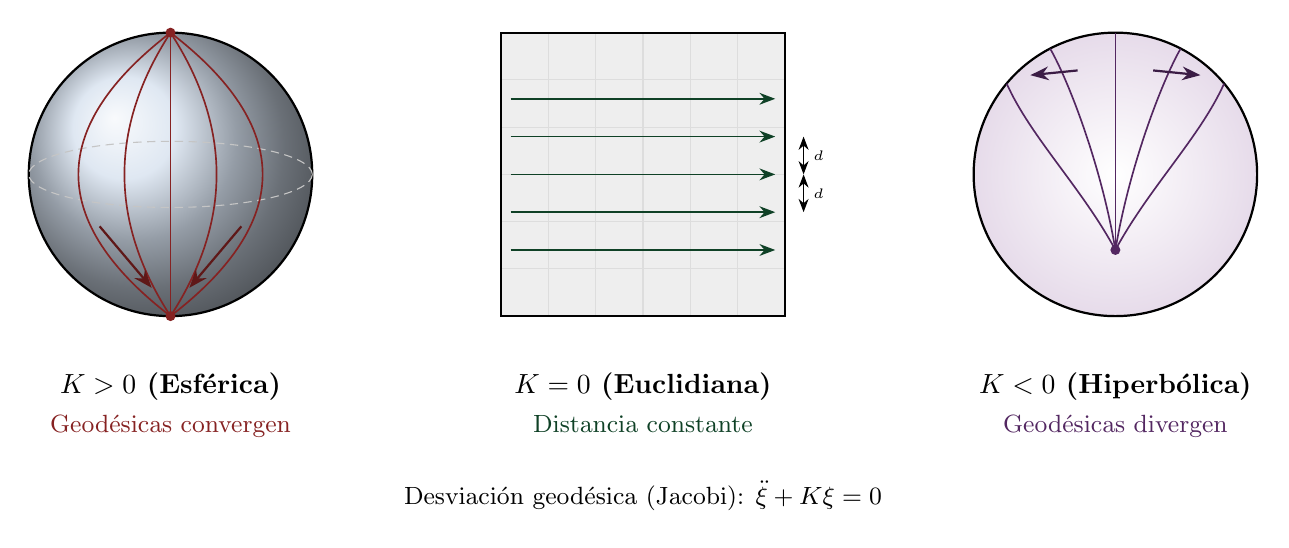
\begin{tikzpicture}[scale=1.2, >=Stealth]

% === Panel 1: K > 0 (Esférica) ===
\begin{scope}[shift={(-5,0)}]
    % Esfera con sombreado 3D
    \shade[ball color=gdlblue!20] (0,0) circle (1.5cm);
    \draw[thick] (0,0) circle (1.5cm);

    % Elipse ecuatorial para efecto 3D
    \draw[gdlgray!50, densely dashed, thin] (0,0) ellipse (1.5cm and 0.35cm);

    % Polos
    \fill[gdlred!70!black] (0,1.5) circle (1.5pt);
    \fill[gdlred!70!black] (0,-1.5) circle (1.5pt);

    % Meridianos (geodésicas que divergen desde el polo norte y convergen en el polo sur)
    \foreach \cx in {-1.3, -0.65, 0, 0.65, 1.3} {
        \draw[semithick, gdlred!70!black]
            (0,1.5) .. controls (\cx,0.5) and (\cx,-0.5) .. (0,-1.5);
    }

    % Flechas indicando convergencia hacia el polo sur
    \draw[->, thick, gdlred!50!black] (0.75,-0.55) -- (0.2,-1.2);
    \draw[->, thick, gdlred!50!black] (-0.75,-0.55) -- (-0.2,-1.2);

    % Etiquetas
    \node[below] at (0,-2) {\textbf{$K > 0$ (Esférica)}};
    \node[below, font=\small, gdlred!70!black] at (0,-2.45) {Geodésicas convergen};
\end{scope}

% === Panel 2: K = 0 (Euclidiana) ===
\begin{scope}[shift={(0,0)}]
    % Plano con grid
    \fill[gdlgray!15] (-1.5,-1.5) rectangle (1.5,1.5);
    \draw[gdlgray!30, step=0.5] (-1.5,-1.5) grid (1.5,1.5);
    \draw[thick] (-1.5,-1.5) rectangle (1.5,1.5);

    % Rectas paralelas equiespaciadas con flechas de dirección
    \foreach \y in {-0.8, -0.4, 0, 0.4, 0.8} {
        \draw[semithick, gdlgreen!50!black, ->] (-1.4,\y) -- (1.4,\y);
    }

    % Marcadores de distancia constante
    \draw[<->, thin] (1.7,-0.4) -- node[right, font=\tiny] {$d$} (1.7,0);
    \draw[<->, thin] (1.7,0) -- node[right, font=\tiny] {$d$} (1.7,0.4);

    % Etiquetas
    \node[below] at (0,-2) {\textbf{$K = 0$ (Euclidiana)}};
    \node[below, font=\small, gdlgreen!50!black] at (0,-2.45) {Distancia constante};
\end{scope}

% === Panel 3: K < 0 (Hiperbólica) ===
\begin{scope}[shift={(5,0)}]
    % Disco de Poincaré con sombreado radial
    \shade[inner color=white, outer color=gdlpurple!18] (0,0) circle (1.5cm);
    \draw[thick] (0,0) circle (1.5cm);

    % Punto de origen de las geodésicas
    \fill[gdlpurple!70!black] (0,-0.8) circle (1.5pt);

    % Geodésica central (recta, pasa por el centro del disco)
    \draw[semithick, gdlpurple!70!black] (0,-0.8) -- (0,1.5);

    % Par interior (extremos sobre el círculo frontera: ángulos ~62.5° y ~117.5°)
    \draw[semithick, gdlpurple!70!black]
        (0,-0.8) .. controls (0.15,0.1) and (0.5,1.0) .. (0.69,1.33);
    \draw[semithick, gdlpurple!70!black]
        (0,-0.8) .. controls (-0.15,0.1) and (-0.5,1.0) .. (-0.69,1.33);

    % Par exterior (extremos sobre el círculo frontera: ángulos ~40° y ~140°)
    \draw[semithick, gdlpurple!70!black]
        (0,-0.8) .. controls (0.35,-0.15) and (0.9,0.4) .. (1.15,0.96);
    \draw[semithick, gdlpurple!70!black]
        (0,-0.8) .. controls (-0.35,-0.15) and (-0.9,0.4) .. (-1.15,0.96);

    % Flechas indicando divergencia
    \draw[->, thick, gdlpurple!50!black] (0.4,1.1) -- (0.9,1.05);
    \draw[->, thick, gdlpurple!50!black] (-0.4,1.1) -- (-0.9,1.05);

    % Etiquetas
    \node[below] at (0,-2) {\textbf{$K < 0$ (Hiperbólica)}};
    \node[below, font=\small, gdlpurple!70!black] at (0,-2.45) {Geodésicas divergen};
\end{scope}

% === Ecuación de Jacobi (anotación global inferior) ===
\node[font=\small] at (0,-3.4) {Desviación geodésica (Jacobi): $\ddot{\xi} + K\xi = 0$};

\end{tikzpicture}
\end{document}
